\dev{Emile Martinez}{}

\textit{Présente en OCamL la correspondance entre les arbres binaires et les arbres généraux. Ce dévellopement peut tout à fait s'insérer dans la leçon sur les arbres, tout comme dans la leçon sur le principe d'induction}

\paragraph{Objectif} Stocker les arbres généraux à $n$ noeuds sous formes d'arbres binaires à $n$ noeuds.

\begin{rem}
	Comment est-ce possible ? Les arbres binaires ne sont ils pas inclus dans les arbres généraux ?\newline
	
	Et bien non, car dans les arbres généraux, il n'y a pas d'arbres vides. En effet,
	\raisebox{-0.5\height}{\begin{tikzpicture}[-, node distance=1cm]
	\node[state, scale=0.4] (q0) {};
	\node[state, below left of = q0, scale=0.4] (q1) {};
	\node[below left of = q1] (q2) {E};
	\node[below right of = q1] (q3) {E};
	\node[below right of = q0] (q4) {E};
	
	
	
	\draw (q0) edge[] node{} (q1) ;
	\draw (q1) edge[] node{} (q2) ;
	\draw (q1) edge[] node{} (q3) ;
	\draw (q0) edge[] node{} (q4) ;


	\end{tikzpicture}} et 
	\raisebox{-0.5\height}{\begin{tikzpicture}[-, node distance=1cm]
	\node[state, scale=0.4] (q0) {};
	\node[state, below right of = q0, scale=0.4] (q1) {};
	\node[below left of = q1] (q2) {E};
	\node[below right of = q1] (q3) {E};
	\node[below left of = q0] (q4) {E};
	
	
	
	\draw (q0) edge[] node{} (q1) ;
	\draw (q1) edge[] node{} (q2) ;
	\draw (q1) edge[] node{} (q3) ;
	\draw (q0) edge[] node{} (q4) ;
	
	
	\end{tikzpicture}} sont différents, alors que pour les arbres généraux, on a un seul arbre à $2$ noeuds 	\raisebox{-0.5\height}{\begin{tikzpicture}[-, node distance=1cm]
	\node[state, scale=0.4] (q0) {};
	\node[state, below of = q0, scale=0.4] (q1) {};
	
	\draw (q0) edge[] node{} (q1) ;
	
	\end{tikzpicture}}
	
\end{rem}

\paragraph{Stratégie} On va stocker un arbre général sous la forme 
\raisebox{-0.5\height}{\begin{tikzpicture}[-, node distance=1cm]
\node[state, scale=0.4] (q0) {};
\node[ below left of = q0] (q1) {1er fils};
\node[below right of = q0] (q2) {frère droit};


\draw (q0) edge[] node{} (q1) ;
\draw (q0) edge[] node{} (q2) ;

\end{tikzpicture}}
ou encore
\raisebox{-0.5\height}{\begin{tikzpicture}[-, node distance=1.2cm]
\node[state, scale=0.4] (q0) {};
\node[ below of = q0] (q1) {1er fils};
\node[right =0.7cm of q0] (q2) {frère droit};


\draw (q0) edge[] node{} (q1) ;
\draw (q0) edge[] node{} (q2) ;

\end{tikzpicture}}

\begin{example}
	\raisebox{-0.5\height}{\begin{tikzpicture}[-, node distance=0.8cm]
	\node[state, scale=0.5] (q0) {0};
	\node[state, below left =0.6cm and 0.6cm of q0, scale=0.5] (q1) {1};
	\node[state, below of = q0, scale=0.5] (q2) {2};
	\node[state, below right of = q0, scale=0.5] (q3) {3};
	\node[state, below left of = q1, scale=0.5] (q4) {4};
	\node[state, below of = q1, scale=0.5] (q5) {5};
	\node[state, below right of = q1, scale=0.5] (q6) {6};
	\node[state, below of = q3, scale = 0.5] (q7) {7};
	
	\draw (q0) edge[] node{} (q1) ;
	\draw (q0) edge[] node{} (q2) ;
	\draw (q0) edge[] node{} (q3) ;
	\draw (q1) edge[] node{} (q4) ;
	\draw (q1) edge[] node{} (q5) ;
	\draw (q1) edge[] node{} (q6) ;
	\draw(q3) edge[] node{} (q7);
	
	
	\end{tikzpicture}} $\quad \longrightarrow \quad$ 	
	\raisebox{-0.5\height}{\begin{tikzpicture}[-, node distance=0.8cm]
	\node[state, scale=0.5] (q0) {0};
	\node[state, below of = q0, scale=0.5] (q1) {1};
	\node[state, right of = q1, scale=0.5] (q2) {2};
	\node[state, right of = q2, scale=0.5] (q3) {3};
	\node[state, below = 1.6cm of q1, scale=0.5] (q4) {4};
	\node[state, right of = q4, scale=0.5] (q5) {5};
	\node[state, right of = q5, scale=0.5] (q6) {6};
	\node[state, below of = q3, scale = 0.5] (q7) {7};
	\node[right of = q0] (E0) {E};
	\node[right of = q3] (E1) {E};
	\node[right of = q6] (E2) {E};
	\node[below of = q2] (E3) {E};
	\node[below of = q4] (E4) {E};
	\node[below of = q5] (E5) {E};
	\node[below of = q6] (E6) {E};
	\node[below of = q7] (E7) {E};
	\node[right of = q7] (E8) {E};
	
	
	\draw (q0) edge[] node{} (q1) ;
	\draw (q1) edge[] node{} (q2) ;
	\draw (q2) edge[] node{} (q3) ;
	\draw (q1) edge[] node{} (q4) ;
	\draw (q4) edge[] node{} (q5) ;
	\draw (q5) edge[] node{} (q6) ;
	\draw (q3) edge[] node{} (q7);
	\draw (q0) edge[] node{} (E0);
	\draw (q3) edge[] node{} (E1);
	\draw (q6) edge[] node{} (E2);
	\draw (q2) edge[] node{} (E3);
	\draw (q4) edge[] node{} (E4);
	\draw (q5) edge[] node{} (E5);
	\draw (q6) edge[] node{} (E6);
	\draw (q7) edge[] node{} (E7);
	\draw (q7) edge[] node{} (E8);
	
	\end{tikzpicture}}
	
	
\end{example}

\begin{rem}
	On remarque que le fils droit de la racine, c'est E. En effet, on a envie de dire que la racine n'a pas de frère droit.
\end{rem}

\begin{lstlisting}
type bin = E | B of int*bin*bin;;

type arbre = N of int*arb_liste 
and
type arb_liste = V | Cons of arbre*arb_liste;;

let rec conversion (arb : arbre): bin = match arb with
  | N(i, E, E) -> B(i, E, E)
  | N(i, Cons(a,l)) -> let B(j, g1, d1) = conversion N(i,l) in
                       let B(k, g2, d2) = conversion a in
                       B(i, B(k, g2, g1), E)
;;
\end{lstlisting}

\begin{center}
	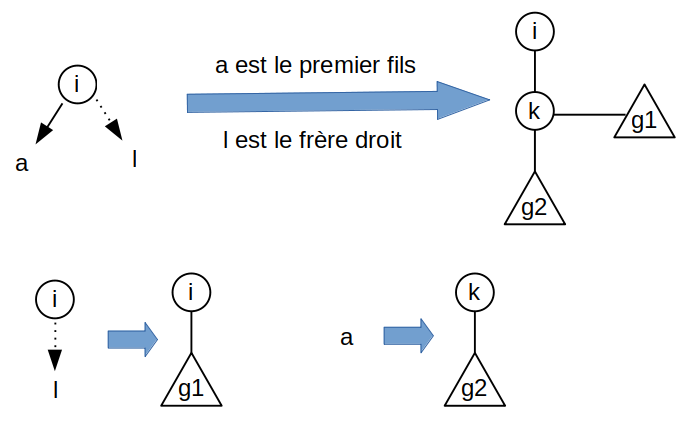
\includegraphics[scale=0.4]{Developpements/Correspondance arbres binaires et généraux/transf_gen_a_bin.png}
\end{center}
Il faut alors montrer que : \begin{enumerate}
	\item conversion est bien définie
	\item conversion N(x, .) est de la forme \lstinline|B(x, . , E )|
	\item conversion est injective
	\item \lstinline{|conversion a| = |a|}
	\item Pour \lstinline|B(x, b, E)|, $\exists$ a : conversion a = \lstinline|B(x, b, E)|
	
\end{enumerate}

Chaque preuve se fera par induction, on ne fera donc pas tout. Montrons 1 et 5. \newline

\begin{proof}Preuve de 1
	
	Montrons par induction sur la structure d'arbre que conversion a termine toujours, et renvoie quelque chose de la forme \lstinline|B( . , . , . )|.\\
	
	$\star$ Cas de bases : conversion(N(x, V)) termine et renvoie B(x, E, E) donc la propriété est vérifié.
	\begin{com}
		On peut dire ici que il n'y a pas de cas de bases pour les arbres, donc on prend le cas de bases pour les la définition des arbres en incluant celles des listes, ce qui nous fait un cas de bases pour les listes.
	\end{com}
	
	\begin{com}
		Pour justifier ce fait là, il faut pointer ce qui se passe et quel code s'exécute sur l'algorithme
	\end{com}

	$\star$ Supposons la propriété d'induction vraie pour N(x,l) et a deux arbres.
	Alors, conversion(N(x,l)) termine et est de la forme B(...) donc le premier let termine.\\
	De même, par propriété d'induction, conversion(a) termine et est de la forme B(...) donc le deuxième let termine.\\
	Donc conversion(N(x,l)) termine t renvoie B(i, B(etc...) ce qui est bien de la forme B(...).\\
	
	Ainsi par induction structurelle, conversion termine toujours.

\end{proof}

\begin{proof}Preuve de 5
	
	Montrons par induction sur la structure d'arbre binaire de b que pour tout $x \in \N$, $\exists$ a : conversion a = B($x$, b, E)
	
	$\star$ Cas de bases : soit $x \in \N$. Alors conversion N($x$, V) = B($x$, E, E). Donc la propriété est vraie sur les cas de bases\\
	
	$\star$ Soient g et d deux arbres binaires vérifiant la propriété.
	Soit $x, y\in \N$. On cherche donc a tel que conversion a = B(x, B(y, g, d), E).
	
	\begin{center}
		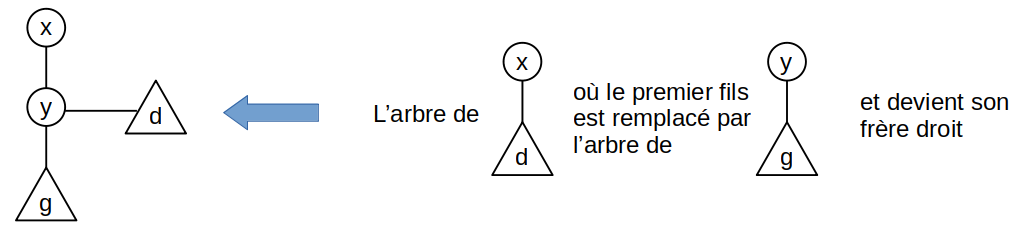
\includegraphics[scale=0.5]{Developpements/Correspondance arbres binaires et généraux/idee_surjectif.png}
	\end{center}
	
	Pa hypothèse d'induction on a qu'il existe un arbre b tel que conversion b = B(x, d, E) et il existe un arbre c tel que conversion c = B(y, g, E).\\
	
	En notant b = N($x$, l) (par 2), on a conversion(N(x, c::l) = B(x, B(y, g, d), E).
	
	\begin{com}
		La il faut montrer pourquoi quand on l'injecte dans l'algo, indéniablement, cela fonctionne, en le faisant étape par étape.
	\end{com}
	
\end{proof}

	\begin{appl}
		On peut utiliser ce code pour encoder les arbres en C par des arbres binaires.
		\begin{com}
			Expliquer à l'oral pourquoi que c'est pratique, que les parcours se font plus facilement, que l'encodage d'un arbre binaire est quand meme bien plus simple qu'un arbre générique.
		\end{com}
		En réalité, notre codage revient au codage en C où mais en plus simple.
		\begin{com}
			Le codage en C étant celui où stocke un arbre comme une valeur et un pointeur vers une liste chaînée, elle même pointant vers les arbres fils. Dans notre transformation, on élude alors le problème de la liste chaînée.
		\end{com}
		\begin{center}
			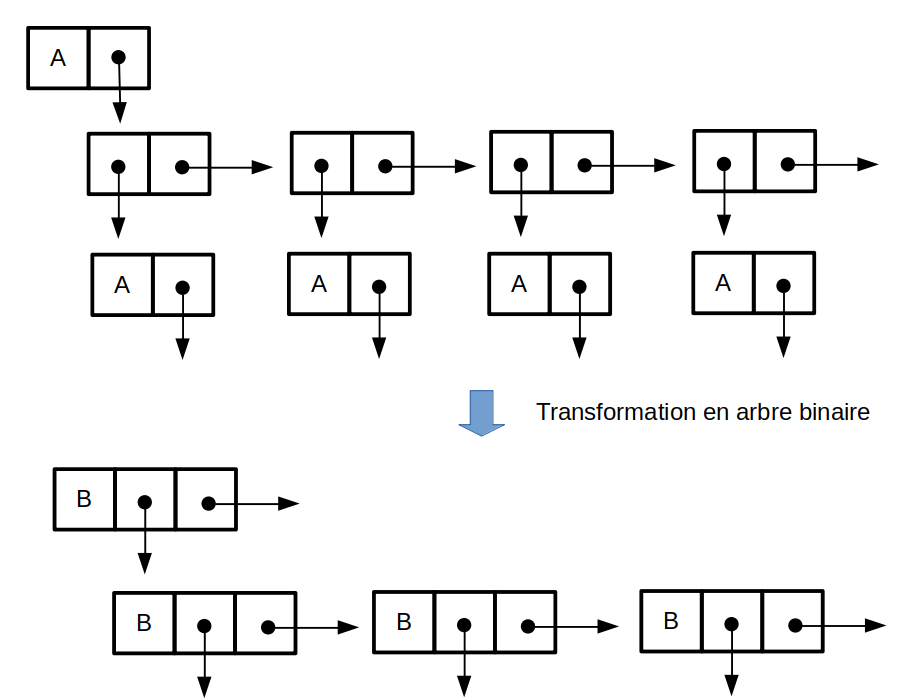
\includegraphics[scale=0.4]{Developpements/Correspondance arbres binaires et généraux/arbre_en_c.png}
		\end{center}
	\end{appl}